%-------------------------------------------------------------------------------
% yum_top_panel
%-------------------------------------------------------------------------------
%
% \file        yum_top_panel.tex
% \library     Documents
% \author      Chris Ahlstrom
% \date        2015-05-29
% \update      2018-05-26
% \version     $Revision$
% \license     $XPC_GPL_LICENSE$
%
%     Provides the Top Panel section of the manual.
%
%-------------------------------------------------------------------------------
\section{Top Panel}
\label{sec:top_panel}

   The \textsl{Yoshimi} top panel provides quick access to some major
   features of the application.
   The top panel is shown in
   \figureref{fig:yoshimi_main_screen}.

   Here are the major elements of the top panel. There have been several
   new additions and a reorganisation of this section starting from
   \textsl{Yoshimi} V 2.2.0.

   \begin{enumber}
      \item \textbf{Stop!}
      \item \textbf{Reset}
      \item \textbf{Stereo}
      \item \textbf{Mixer Panel}
      \item \textbf{Virtual Keyboard}
      \item \textbf{Midi Learn}
      \item \textbf{Vectors}
      \item \textbf{Undo}
      \item \textbf{Redo}
      \item \textbf{Detune}
      \item \textbf{Volume}
      \item \textbf{Key Shift}
      \item \textbf{F. BPM}
   \end{enumber}

   \setcounter{ItemCounter}{0}      % Reset the ItemCounter for this list.

   \itempar{Stop!}{top panel!stop all sound}
   Stop!
   This button causes \textsl{Yoshimi} to
   "Cease all sound immediately!"
   Useful when MIDI input suddenly stops, resulting in 'stuck' notes, most
   likely due to a bug in the MIDI source.

   \itempar{Reset}{top panel!reset}
   \index{master reset}
   Master Reset.
   Resets \textsl{Yoshimi} to its default state, when no default configuration
   files exist.  If there is a saved default state and the \textbf{start with
   default} option is set, then a reset will reload that file. For any other
   situation it will set the first-time defaults.

   \index{master reset, ctrl}
   If the Ctrl key is held down while doing a master reset, then
   MIDI Learn will also be cleared.

   \itempar{Stereo}{top panel!stereo}
   Stereo Button.
   This toggles the main audio output between stereo and mono, but doesn't
   affect individual part ones.
   It is useful for checking balance between the two on the fly while playing.
   This is new from V 1.5.11.

   \itempar{Mixer Panel}{top panel!mixer panel}
   This button brings up a panel that shows a "mixer" view
   of all of the parts that have been created in the current
   state of \textsl{Yoshimi}.

   For the details of this panel,
   see \sectionref{subsec:mixer_panel_window}.

   \itempar{Virtual Keyboard}{top panel!virtual keyboard}
   This button brings up the virtual keyboard, which is a way to enter
   MIDI information without a real MIDI keyboard.
   It also provides a way to use the computer keyboard for faster
   playing.  See \sectionref{subsec:virtual_keyboard}.

   \itempar{Midi Learn}{top panel!midilearn}
   When pressed, the \textsl{Yoshimi} Midi Learn editing window is opened.
   This button used to be for opening the \textsl{Yoshimi} Reports window,
   but that is seldom changed so they've been swapped.

   \itempar{Vectors}{top panel!vectors}
   Provides two or four part vector control.  This was originally in the \textbf{Yoshimi} menu.  See
   \sectionref{subsec:vector_dialogs}.

   \itempar{Undo}{top panel!undo}
   Undo Button.
   This reverts the last control change made. More details are found in \sectionref{subsec:undo_redo}.
   This is new from V 2.2.0.

   \itempar{Undo}{top panel!redo}
   Redo Button.
   This re-applies control change that was most recently 'undone'.
   More details are found in \sectionref{subsec:undo_redo}.
   This is new from V 2.2.0.

   \itempar{Detune}{top panel!detune}
   Detune.  Provides a global fine detune functionality.
   The fine detune mapping to the knob values shown below is
   -64 to 63 cents.

   Values: \texttt{0 to 127, 64*} (float)

   \itempar{Volume}{top panel!overall volume}
   Volume, Master Volume.
   Controls the overall volume of all sounds generated by
   \textsl{Yoshimi}.

   Values: \texttt{0 to 127, 90*}

   \itempar{Key Shift}{top panel!key shift}
   Master Key Shift.
   This is the key-shift (transpose) that applies to all parts, in units of
   semitones.
   In recent versions of \textsl{Yoshimi}, this range has been extended.
   Also note that the master key shift can be set via the user-interface, the
   command-line, or by MIDI NRPN commands.

   Values: \texttt{-36 to 36, 0*}

   Also see the \textbf{Key Shift} item in
   \sectionref{sec:bottom_panel}\hspace{6 pt}for more information.


   \itempar{F. BPM}{top panel!fallback bpm}
   Fallback BPM.
   Provides a synchronising MIDI clock for BPM controls if
   \textsl{Yoshimi} is not seeing an incoming one.
   This is new from V 2.2.0.

   Values: \texttt{32 to 480, 120*}

\subsection{Mixer Panel Window}
\label{subsec:mixer_panel_window}
\index{Panel}

   The \textsl{Mixer Panel} button opens the "Mixer" window.
   The mixer provides a global view of the most important
   adjustable parameters of all of the defined parts.
   There are two views, a 2x8 view and a 1x16 view.
   See \figureref{fig:yoshimi_part_panel_1x16}, which
   shows the 1x16 view.

   The Mixer Panel Window acts like a mixer and allows one to edit some important
   part parameters, such as Instrument choice, Volume, Panning, etc.\\
   Also, since V 1.5.11 this window shows VU-meters for each part.
   To make a part the current part, left-click on its \textbf{Edit} button.
   To edit an instrument, right-click on the \textbf{Edit} button for that
   instrument.

   When using the JACK audio backend, parts can be individually routed or sent
   to the main L/R outputs, either by themselves, or working with the main Left
   and Right outputs at the same time.  This is controlled from the panel
   window, and the settings are saved with all the other parameters.

   The individual \textsl{Direct Part} outputs will have the part effects, and any
   \textbf{Insertion} effects that are linked to them, but not the
   \textbf{System} effects.

   \textsl{Yoshimi} used to register all parts with JACK by default, but that
   is a bit much now that 64 parts are available, so now \textsl{Yoshimi}
   uses an "on demand" model.

   In the mixer panel window one will see a field just above the
   \textbf{Edit} button.
   This field determines the audio destination on a part-by-part basis,
   defaulting to just the main L+R pair. The direct part outputs are only
   exposed on parts that are active, and have the destination set to either
   \textbf{part} or \textbf{both}.
   Once activated, they will remain in place for the entire session, even if
   the part is later disabled or routed to main only. This is so that other
   programs won't see links suddenly disappear, although they will become
   silent.  This setting is preserved in Yoshimi's patch sets and will be
   re-instated when next loaded.

\begin{figure}[H]
   \centering
   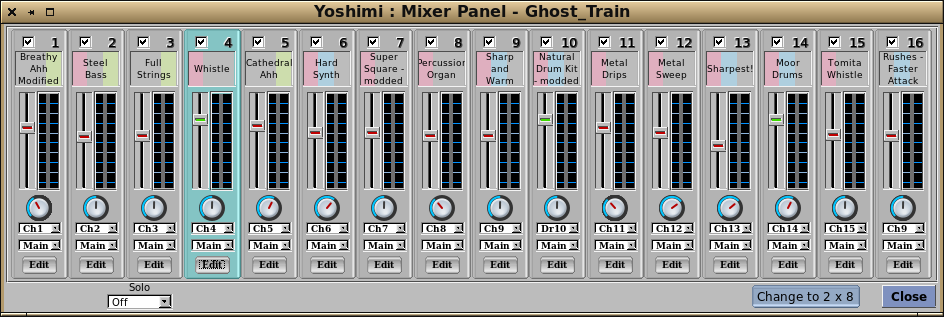
\includegraphics[scale=0.5]{2.3.3/mixer.png}
   \caption[Yoshimi Mixer Panel]{Yoshimi Mixer Panel, 1x16 View}
   \label{fig:yoshimi_part_panel_1x16}
\end{figure}

   Note that there is also a 2x8 version of this dialog (not shown).
   This dialog has been further updated; as well as the \textbf{Solo}
   control, (described below) it now presents separate left and right
   VU meter bars.

   \setcounter{ItemCounter}{0}      % Reset the ItemCounter for this list.

   \itempar{Part Summary}{Part Section, 1 to 16}
   Parts View or Summary.

   \itempar{Enable part}{parts!enable}
   Enable/Disable the part. The check-box enables/disables the part.
   When the part is disabled, its controls are greyed out.

   Values: \texttt{Off*, On}

   \itempar{Part name}{parts!name}
   Instrument name. Click on this box to change the instrument (it will
   open up the current \textbf{Bank} window if it wasn't already open.

   \itempar{Volume Slider}{parts!volume}
   Volume Bar.
   Changes the volume of the part.

   \itempar{VU-meter display}{parts!meter}
   Shows the level of the part when playing.

   \itempar{Panning Knob}{parts!panning}
   Panning Dial-Button.
   Changes the panning of the part.

   Values: \texttt{0 (left) to 64* (center) to 127 (right)}

   \itempar{Channel}{parts!channel}
   Receive from MIDI channel.
   Changes the MIDI channel assigned to the part.

   Values: \texttt{Ch1*, Ch2, ..., Ch16}

   \itempar{Main}{parts!destination}
   Set Audio Destination.
   Sets the audio for this part to be routed to the main audio output, to
   the audio specified by the part setup, or to both outputs.
   This option requires that \textsl{Yoshimi} use JACK audio.  If running
   ALSA, this option is disabled (greyed out).
   The part's audio destination (JACK) is saved with the patch sets, and
   so is the number of available parts.

   Values: \texttt{Main, Part, or Both}

   \itempar{Edit}{parts!edit}
   The Edit button provides two functions.
   \begin{itemize}
      \item Left mouse button: Makes this the currently selected part.
      \item Right mouse button: As above, but also opens the part edit window.
   \end{itemize}
   This setup is a bit unintuitive, but the tooltips make it clear
   which click one might want to use.

   \itempar{Solo}{parts!solo}
   \index{channel switcher}
   \index{parts!channel switcher}
   There are several basic commands that change the way
   \textsl{Yoshimi} responds to incoming MIDI,
   so that only one of a group of instruments will see note-on events, but all
   of the group will see note-off ones. These commands
   are in the \textbf{Mixer Panel}, as shown below.
\begin{figure}[H]
   \centering
   
\includegraphics[scale=0.55]{2.3.0/solo.png}
   \caption[Yoshimi Mixer Panel]{Yoshimi Mixer Panel, Solo}
   \label{fig:yoshimi_part_panel_solo}
\end{figure}
   They are referred as a \textsl{Solo} feature.
   The \textbf{Solo} settings are saved in patch sets, which saves a
   little frustration when loading one's current favourite patch set.

   Since \textsl{Yoshimi} V 1.7.1 a new mode of operation has been available, so the complete list is:

   Values: \texttt{Off*, Row, Column, Loop, TwoWay, Channel}

   For these modes, if one has a programmable MIDI controller, one can set it
   up to activate a specific part, or to increment/decrement which part in the
   set is active.  The \textbf{Solo} drop-down list enables the feature for
   one of these modes, and also makes the CC spin-box visible.
   One uses this spin-box to set which incoming CC changes the part that gets
   new notes.
   The \textsl{value} this CC sends performs the actual change, instantly and
   silently. Most importantly it leaves any existing notes sounding, though a
   note off will release them and set the effects tail.

   \index{solo!row}
   \textbf{Row} means that all of the first 16 channels will be set to channel
   1, but with only one active, and one's CC will dial up any of the parts,
   disabling the others.
   In \textbf{Row} mode the whole of the first 16 parts are ostensibly
   receiving on channel 1.  This mode is most useful if one wants to play live
   through a piece with multiple instrument changes while playing. It works
   best with a foot switch that internally stores a channel number and
   increments/decrements it with every press, then sends it.

   Although this uses all of the first 16 parts, one can set the number of
   parts to 32, so that one can use the 17+ row for normal 1 through 16
   channels. Also, if one has \textbf{vector control} set up, \textbf{Solo}
   intelligently recognises this fact, and, for each vector it finds, it will
   switch in/out the whole vector column appropriately.

   \index{solo!column}
   For running \textbf{Solo} in \textbf{Column} mode, one needs to have 32 or
   (preferably) 64 parts set; with this setup, one can have up to 4 parts
   switched per channel, and independently of each other. However, this works
   more like vector control in that switching has to be in groups of 16. For
   example, to control the channel 4 column one would send 4, 20, 36, 52 to
   select the wanted part. This usage is more appropriate for post recording
   MIDI automation.

   For both of these modes, if one has a programmable MIDI controller, one can
   set it up to activate a specific part, or the increment/decrement which part
   in the set is active.

   Note that \textbf{Row and Column} are recommended only for automation.

   \index{solo!loop}
   \textbf{Loop}.  Loop mode is a variation on the Row mode.
   With this mode, if one sends \textsl{any} value (except zero)
   via the designated CC,
   it will increment the active part by one, rolling round to 1 after 16.
   This should make even the dumbest foot controller usable.

   To keep it all lightweight, one needs to load and activate all the patches
   and parts wanted, but that could be obtained from a saved patch set, and the
   channels are only changed from the very first time one sends the CC.  To
   look really clever, the whole lot can be embedded in a MIDI file.

   One can play a piece that needs to live-switch between 10 instruments, using
   a footswitch to do the channel changes. The device holds a channel
   number (starting with zero) and increments/decrements it depending on which
   switch is pressed, then sends the resulting CC.

   At the \textsl{2017 Linux Audio Conference},
   it became obvious there was a possible problem with the \textbf{Loop}
   feature. This issue arose from the 'bounce' of a cheap footswitch that would
   then send two changes instead of one. It is now resolved by adding a
   debounce timer of about 60ms so that a second pulse inside that time will be
   ignored.

   \index{solo!TwoWay}
   \textbf{TwoWay}.
   A further development suggested at that time has now also been implemented. This
   is the addition of a \textbf{TwoWay} option.
   This option works in a similar way to \textbf{Loop}, but
   a value between 1 and 63 will step down instead of up, so that if one does make
   a mistake it can quickly be rectified.

   With a reasonable MIDI controller one can usually set a couple of foot switches
   to report the same CC but with different values. Alternatively stick to their
   native values and pass them through something like \textsl{QmidiRoute} to do the
   translation.

   \index{solo!Channel}
   \index{new!Solo Channel}
   \textbf{Channel}.
   This new mode of operation will block new notes sent to all parts that are not
   on the same MIDI channel as the one sending the CC if the value sent on the
   designated CC is greater than 63. Note Off messages will still be seen. If the
   CC value is less than 64, these other parts will be re-enabled again.

   If the same CC is sent on a different channel, then the new one will cancel the
   old one and become the soloed one. It follows on that any channel can cancel the
   feature.

   \itempar{Parts Layout}{parts!change layout}
   \index{parts!2x8}
   \index{parts!1x16}
   Changes the layout of the panel to the other layout, either
   \textbf{Change to 2 x 8} or
   \textbf{Change to 1 x 16}.

   \itempar{Close}{parts!close}
   Close the window.

\subsection{Undo Redo}
\label{subsec:undo_redo}
\index{Undo Redo}
   These two controls provide one with the ability to correct mistakes, or simply
   switch between different settings to see which works best.
   There is some intelligence built in. For example, adusting a control several
   times without actually playing a note, will only store the last change made.

   There are also some group settings. A good example is in the resonance window.
   Here, if one uses the Rnd1, Rnd2, Rnd3 buttons then Undo and Redo will reset
   the entire graph. However changing the resonance shape by dragging in the graph
   itself makes a series of point-by-point changes which would then have to be
   undone/redone one at a time.

   If one has stepped back through the undo stack and then alters a control, it is
   no longer possible to redo any of the settings that were made after that one
   was originally made, but all settings prior to this can still be undone.

   A few settings would be impractical, or even impossible to undo. In these
   cases one is warned this is so, and that the entire undo stack will have to
   be cleared if one proceeds.

\subsection{Virtual Keyboard}
\label{subsec:virtual_keyboard}

   This section describes the detailed usage of the
   \textsl{Yoshimi} virtual keyboard.
   The virtual keyboard lets one play notes using the keyboard/mouse. There is
   no MIDI requirement.

   Using the computer keyboard: The keyboard is split into three octaves.
   It may happen that the keys will not trigger a note-on;
   this happens when another widget has the keyboard focus.
   To play using the computer keyboard, click on the virtual keyboard.

   Using the mouse: One can use the mouse to play.  If one presses the
   Shift key while pressing the mouse button, the keys will not be released
   when the mouse button is released.  If one presses the \textbf{Stop!} or
   "panic" button from the \textsl{Yoshimi} main window,
   all keys are released.

\begin{figure}[H]
   \centering
%  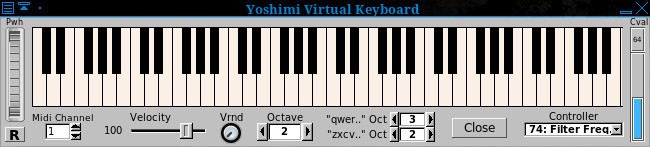
\includegraphics[scale=1.0]{top-panel/yoshimi-virtual-keyboard.jpg}
   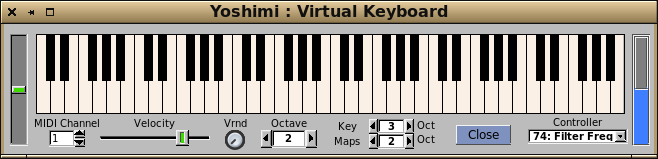
\includegraphics[scale=1.0]{2.3.0/keyboard.png}
   \caption{Yoshimi Virtual Keyboard}
   \label{fig:yoshimi_virtual_keyboard}
\end{figure}

\subsubsection{Virtual Keyboard, Basics}
\label{subsubsec:virtual_keyboard_basics}

   \begin{enumber}
      \item \textbf{Pwh}
%     \item \textbf{R}
      \item \textbf{Midi Channel}
      \item \textbf{Velocity}
      \item \textbf{Vrnd}
      \item \textbf{Octave}
      \item \textbf{Key Oct}
      \item \textbf{Maps Oct}
      \item \textbf{Controller}
      \item \textbf{Cval}
      \item \textbf{Close}
   \end{enumber}

   \setcounter{ItemCounter}{0}      % Reset the ItemCounter for this list.

   \itempar{Pwh}{vkdb!pitch bend}
   Pitch bend knob. Pitch wheel.
   This item is now a slider control.  To reset it to the middle position,
   right-click within the slider.
   \itempar{Midi Channel}{vkdb!midi channel}
   MIDI Channel.
   Sets the MIDI channel for the virtual keyboard.

   Values: \texttt{1* to 16}

   \itempar{Velocity}{vkdb!velocity}
   Velocity of Notes.
   Sets the note-on velocity for the virtual keyboard.

   Values: \texttt{1 to 127, 100*}

   \itempar{Vrnd}{vkdb!velocity randomness}
   Velocity Randomness.

   Values: \texttt{0* to 127}

   \itempar{Octave}{vkdb!qwerty}
   Transposes all of the virtual keyboard notes by the given number of
   octaves.

   Values: \texttt{1, 2*, 3, 4, 5}

   \itempar{Key Oct}{vkdb!key octave}
   Transposes the upper keys (the numbers and the "qwert" keys);
   the range of these keys is from C-4 to A-5 (replace the '5' with the octave).
   Look at the tooltips as a reminder.

   Values: \texttt{1, 2*, 3, 4, 5}

   \itempar{Maps Oct}{vkdb!maps octave}
   Transposes the lower keys ("sdghj" and "zxcvb"); the range of these keys is
   from C-3 to E-4 (replace the '4' with the octave).  Look at the tooltips as a
   reminder.

   Values: \texttt{1, 2*, 3, 4, 5}

   \itempar{Controller}{vkdb!controller}
   Keyboard Controller.
   \begin{quote}
   Values:\\
   \texttt{01:Mod.Wheel, 07:Volume, 10:Panning,
      11:Expression, 64:Sustain, 65:Portamento, 71:Filter Q,
      74:Filter Freq*, 75:Bandwidth, 76:FM Gain,
      77:Res.c.freq, 78:Res.bw.}
    \end{quote}

   Sets the controller to be changed according to the \textbf{Cval}
   controller.
   See \sectionref{subsubsec:virtual_keyboard_controllers}.

   \itempar{Cval}{vkdb!controller value}
   Controller value.
   Changes the controller value.
   This item is a combination value-bar and slider that one
   can move up and down with the mouse, to change the controller value. The
   numeric value is indicated with a dynamic tooltip. Note that the value might
   not reflect the internal value of the controller when one changes the
   controller. The default value changes depending on the controller type.

   Values: \texttt{1 to 127}

   \itempar{Close}{vkdb!close}
   Close button.

\subsubsection{Virtual Keyboard, ASCII Mapping}
\label{subsubsec:virtual_keyboard_ascii}

   In addition to this virtual keyboard, the QWERTY (or Dvorak, or AZERTY)
   keyboards can be used to produce notes.
   The computer keyboard layout is shown in
   \figureref{fig:qwerty_virtual_keyboard},
   The "white" keys are the light shade, and the "black" keys are the
   darker shade.
   The range of the keys on the "zxcvb..." row is C3 to E4.
   The range of the keys on the "qwert..." row is C4 to A5.
   These octave ranges can be adjusted.
   The computer keyboard will produce notes only when the virtual keyboard
   has focus.
%  Also note that we replaced the monopoly symbol with the monopolist
%  symbol.  On X11 systems, this key is known as the "Super" key.

\subsubsection{Virtual Keyboard, Controllers}
\label{subsubsec:virtual_keyboard_controllers}

   This section gives a brief overview of the controller's that this
   window supports.

   \begin{enumber}
      \item \textbf{01: Mod. Wheel}
      \item \textbf{07: Volume}
      \item \textbf{10: Panning}
      \item \textbf{11: Expression}
      \item \textbf{64: Sustain}
      \item \textbf{65: Portamento}
      \item \textbf{71: Filter Q}
      \item \textbf{74: Filter Freq.}
      \item \textbf{75: Bandwidth}
      \item \textbf{76: FM Gain}
      \item \textbf{77: Res. c. freq}
      \item \textbf{78: Res. bw.}
   \end{enumber}

      The following figure shows the corresponding drop-down list of controller
      values, each preceded by its MIDI control number, the default being 74: Filter Freq.

\begin{figure}[H]
   \centering
%  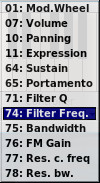
\includegraphics[scale=0.75]{menu/Instrument/virtual-keyboard-controllers.jpg}
   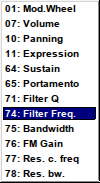
\includegraphics[scale=0.75]{top-panel/virtual-keyboard-controller.png}
   \caption{Virtual Keyboard Controllers}
   \label{fig:virtual_keyboard_controllers}
\end{figure}

   \setcounter{ItemCounter}{0}      % Reset the ItemCounter for this list.

   \itempar{Mod. Wheel}{controllers!modulation wheel}
   Sets the MIDI modulation value.  This control will
   only have an effect on certain instruments.  (It has no effect on the
   "Simple Sound", for example).

   \itempar{Volume}{controllers!volume}
   Controls the overall volume of the instrument being played by the virtual
   keyboard.

   \itempar{Panning}{controllers!panning}
   Controls the left-right location of the sounds played by the virtual
   keyboard.

   \itempar{Expression}{controllers!expression}
   Controls the expression.  This probably can have different effects depending
   on the instrument.  For example, with the "Simple Sound", this control is a
   lot like volume.

   \itempar{Sustain}{controllers!sustain}
   Controls the sustain duration.  This works even with the "Simple Sound".
   Using it makes even this virtual keyboard capable of some "virtuoso"
   expression.

   \itempar{Portamento}{controllers!portamento}
   Controls the time of transition from one pitch to another.
   Using it makes even this virtual keyboard capable of some "virtuoso"
   expression.

   \itempar{Filter Q}{controllers!filter q}
   Controls the sharpness of the filters used in an instrument.
   Generally requires a complex instrument to take effect.
   For example, try this control with the "Weird Pad" instrument in the
   "Fantasy" bank.

   \itempar{Filter Freq}{controllers!filter frequency}
   Controls the center frequency of the filters used in an instrument.
   Generally requires a complex instrument to take effect.
   For example, try this control with the "Weird Pad" instrument in the
   "Fantasy" bank.

   \itempar{Bandwidth}{controllers!bandwidth}
   Controls the frequency bandwidth of the filters used in an instrument.

   \itempar{FM Gain}{controllers!fm gain}
   TODO.
   Haven't found a sound that exercises this control.
   Haven't looked all that hard yet.

   \itempar{Res. c. freq}{controllers!resonance center frequency}
   Resonance Center Frequency.
   Applies only if the part has resonance set up.

   \itempar{Res. bw}{controllers!resonance bandwidth}
   Resonance Bandwidth.
   Applies only if the part has resonance set up.

%-------------------------------------------------------------------------------
% vim: ts=3 sw=3 et ft=tex
%-------------------------------------------------------------------------------
